% general package(s)
\documentclass[12pt]{article}
\usepackage[margin=0.8in]{geometry}
\usepackage[utf8]{inputenc}
\usepackage[english]{babel}
\usepackage[T1]{fontenc}

% math package(s)
\usepackage{amsmath}
%\usepackage[urw-garamond]{mathdesign}
\usepackage{gensymb}

% figure package(s)
\usepackage{booktabs} % For tables
\usepackage{caption} % For subfigures
\usepackage{enumerate}
\usepackage{float}
\usepackage{graphicx}
\usepackage{listings}
\usepackage{subcaption} % For subfigures
\usepackage{wrapfig} % For inline figures

% reference package(s)
\usepackage[capitalize]{cleveref}

% misc. package(s)
\usepackage{color}

\begin{document}
%{\makebox[\textwidth][s]
\title{IEA Task 37 on System Engineering in Wind Energy \\
\large The Wind Farm Physics Model and Optimization Case Studies}
\author{Nicholas F. Baker\thanks{Masters Student, Department of Mechanical Engineering},\  Andrew P. J. Stanley\thanks{Ph.D. Candidate, Department of Mechanical Engineering}, \ Jared Thomas\thanks{Ph.D. Student, Department of Mechanical Engineering}, \ and Andrew Ning\thanks{Assistant Professor, Department of Mechanical Engineering} \\
    {\normalsize\itshape Brigham Young University, Provo, Utah 84602.}\\
Katherine Dykes\thanks{Senior Engineer, National Wind Technology Center}\\
   \normalsize\itshape National Renewable Energy Laboratory, Golden, Colorado 80401}
%\date{June 2018}
\date{\vspace{-5ex}}

\maketitle{}
\vspace{-0.5cm}
\tableofcontents

\section{Introduction}

In order to better understand the effects of different Engineering Wake Model (EWM) selection and optimization algorithm implementation, this document defines two simple wind farm layout optimization (WFLO) case studies. These studies are designed to involve a broad spectrum of participants working on the WFLO problem.
    
    Two of the major factors that effect the results of wind farm layout studies are 1) EWM characteristics and 2) optimization approach. The two below case studies are designed in an attempt to quantify the effects of both choices. The first case study (called the Optimization Only Case Study, described in \cref{Sec:OptOnly}) explores different optimization techniques paired with a simplified EWM. The second case study (called the Combined Physics Model/Optimization Algorithm Case Study, described in \cref{Sec:Cmbnd}) observes the effects of various combinations of EWM and optimization method combination.\footnote{Comparisons just between EWMs does not involve optimization and multiple studies already exist in this area.}
    
    As a participant, your task is to discover the optimal turbine placement for each farm, that delivers the highest AEP possible. For the Optimization Only Case Study, AEP will be calculated by our supplied wake model and algorithm. For the Combined Case Study you are to use your preference of EWM to discover optimal turbine placement, and we will use a Large Eddy Simulator (LES) to calculate and compare AEP of all participant results. You will report both your optimal turbine locations for each wind farm, and describe your methods for finding them in a way that will enable reproducability of your results, the format of which is in \cref{Sec:RepResults}. 
    
    The wind farm characteristics of these two cases are similar, and were selected to be both restrictive enough to maintain simplicity, yet general enough to aid in solving and interpreting the results of more complex and realistic problems.

%\newpage
\section{Problem Definitions}
\subsection{The Optimization Only Case Study}\label{Sec:OptOnly}
    The intent of this case study is to determine best optimization practices when given an EWM that permits both gradient-based and gradient-free methods to be used. As a representative EWM, we select a simplified version of Bastankhah's Gaussian wake model \cite{Thomas2018,Bastankhah2014,Bastankhah2016}. We supply a Python implementation of this wake model, as well as a description of the model in \cref{app:WakeModel} for those who wish to implement it in another language.
    %Reword above and below paragraphs to clarify AEP calculation is defined.

    With the wake model fixed, participants are free to use whichever computational optimization strategies they choose, with the objective of obtaining the maximum Annual Energy Production (AEP) for the defined farm. In this case study the wind farm boundaries, directional wind frequency, wind turbine attributes, and wake model physics are fixed---turbine locations are the only design variables participants are permitted to alter.
    
    Since problem size strongly affects optimization algorithm performance, three wind farms of increasing size are specified in \cref{Sec:OptWindFarm}. These scenarios, roughly doubling in number of turbines, exist to avoid a bias towards algorithms optimized for wind farms of a specific dimension, and in order to observe how increased complexity correlates to algorithm performance. Perfect squares are used to permit grid turbine arrangements, if desired.
    
    The goal of this collaboration is to compare participant results when using different optimization strategies under a single wake model, in order to understand the performance differences resulting from optimization algorithm selection in similar scenarios. While the provided wind farm scenarios are very simple, we expect the results to assist researchers in understanding the differences that occur in WFLO due to various numerical methods. A greater understanding of the trade-offs in algorithm selection for this simplified problem is expected to aid in solving and interpreting the results of more complex and realistic problems.

\subsubsection{Wind Farm Definition}\label{Sec:OptWindFarm}
There are three (3) wind farm size scenarios which will be optimized by all participants:

        \begin{enumerate}
            \item Wind farm of sixteen (16) turbines,
                boundary radius of 1,300 m.
            \item Wind farm of thirty-six (36) turbines,
                boundary radius of 2,000 m.
            \item Wind farm of sixty-four (64) turbines,
                boundary radius of 3,400 m.
        \end{enumerate}
    
    For all wind farm sizes, the wind farm boundary is circular, as depicted \cref{fig:EmptyFarm}. The origin is at the center of the farm, coincident with the depicted reference turbine, and the specified boundary radius for each farm is measured from the origin. The radii magnitudes were determined by evenly distributing the specified number of turbines in concentric circles, with no less than 5 diameter spacing between adjacent turbines, and rounding up to the nearest 100 m.
    
    All wind farms will be populated with the IEA37 3.35 MW onshore reference turbine \cite{NREL335MW}, whose main attributes are summarized in \cref{App:NREL335MW}.
    
    Note that the farm boundary restricts only turbine hub locations. The blade radius is permitted to extend beyond, but hub locations must be on or within the boundary. Hub locations are further restricted from being placed closer to each other than two diameters apart.
    
    \begin{figure}[H]
        \centering
        \includegraphics[width=.65\linewidth]{EmptyOptField.png}
        \caption{Depiction of circular farm boundary with 3,400 m radius. Reference turbine (to scale) placed at origin.}
        \label{fig:EmptyFarm}
    \end{figure}
    
%\newpage
\subsubsection{Baseline Layouts}\label{Sec:Baseline}
To assist in validation, a baseline wind turbine layout is supplied as a check for each farm size. The AEP for these baseline layouts, as determined by our wake model implementation, is included in the \texttt{.csv} file for each size scenario, listed in the \texttt{.zip} file accompanying this document. If you choose to utilize your own implementation of the wake model and AEP functions described in \cref{app:WakeModel} instead of the Python implementation provided, ensure that your implementation reports the same AEP for these locations.

You are also to conduct a single baseline optimization from these baseline layouts, and report your resulting optimized turbine location and AEP values from these starting locations. You are not required to start \textit{each} of your optimizations from these layouts, only report the results from a single run using these starting baselines. For your other optimization attempts, feel free to use random starts, warm starts, intuition, or any other selection method you choose to initialize turbine locations. The exact coordinates for the turbine locations in each of these baseline layouts are also included in \texttt{.csv} files listed in the \texttt{.zip} file accompanying this document. The format for these files is described later in \cref{Sec:Csv}. The baseline layouts are depicted graphically in \cref{fig:BaseLocOpt}

    \begin{figure}[H]
    \centering
        \begin{subfigure}[t]{.49\textwidth}
        \centering
            \includegraphics[width=\linewidth]{BaseCase16.png}
                \caption{16 Turbine Farm} \label{fig:BaseLoc16}
            \end{subfigure}
            %
            \begin{subfigure}[t]{.49\textwidth}
            \centering
            \includegraphics[width=\linewidth]{BaseCase36.png}
            \caption{36 Turbine Farm}\label{fig:BaseLoc36}
            \end{subfigure}
            
            \medskip
            
            \begin{subfigure}[t]{.49\textwidth}
            \centering
            \vspace{0pt}% set the real top as the top
            \includegraphics[width=\linewidth]{BaseCase64.png}
            \caption{64 Turbine Farm} \label{fig:BaseLoc64}
        \end{subfigure}
        %
        \begin{minipage}[t]{.49\textwidth}
            \vspace{20pt}
            \caption{Baseline turbine locations, depicted with dashed wind farm boundaries and blue NREL 3.35 MW onshore reference turbines (to scale)}
            \label{fig:BaseLocOpt}
        \end{minipage}
    \end{figure}

        %\item The wind turbulence intensity is 0.075.
        %\item Assume the freestream wind speeds given in this document are at hub height. If you need a wind shear, use a power law relationship with a shear exponent of 0.15.

\subsubsection{Wake Model and Code Description}
The wake model implemented in this case study is Bastankhah's Gaussian wake model \cite{Thomas2018, Bastankhah2014, Bastankhah2016}. A description of the model's governing equations, data on the wind farm's wind speed and direction probability, and formulations for AEP calculations are included in \cref{app:WakeModel}. The pertinent equations are coded in Python, and are provided alongside this document in a \texttt{.zip} directory, in order for each participant to focus on the optimization aspect and apply their unique methods.

The wake model routine takes turbine grid locations as inputs, and returns as output a single AEP value calculated from the input turbine locations.

Though not necessary, alteration to the released Python code is permitted, if required to maximize optimizer effectiveness. Care must be taken, however, that the governing physics equations are not altered to deliver deviated AEP results. For this reason, baseline turbine locations and AEP calculations are described in \cref{Sec:Baseline}, to be used for validation.

\subsection{The Combined Physics Model/Optimization Algorithm Case Study}\label{Sec:Cmbnd}
    This case study closely matches the one described in \cref{Sec:OptOnly}, with the exception that no wake model is provided, and only a single wind farm size is to be optimized. Participants are free to chose their preferred EWM and optimization method. The objective is to obtain the maximum Annual Energy Production (AEP) for the defined turbine farm. Participants will adjust resultant AEP through choice of EWM utilized, and manipulation of turbine locations.
    
    The intent of this case study is to determine best EWM selection and optimization practices for this representative wind farm scenario.  Since different EWMs approximate the aerodynamic characteristics effecting power production differently, reported AEP from participants using different EWMs are not comparable. As a benchmark measuring tool for these case studies, we will run all participant results of optimized turbine locations through a Large Eddy Simulation (LES). Using LES as a tool for analysis, participant results will be analyzed based on which participant results (regardless of EWM used) give the highest LES-calculated AEP.

    Like the previous case study defined in \cref{Sec:OptOnly}, the wind farm boundary for this case study is circular, and the number of turbines in the farm is a perfect square in order to permit a grid arrangement, if desired. To limit the LES computation time required for us to assess results, the wind farm size for this case study is limited to 9 turbines.
    
    This study differs from the first, in that it assesses not only the optimization methods measured by previous case, but also the effects that different physics model approximations have on turbine location recommendations. While the provided wind farm is very simple, we expect the results to assist researchers in understanding the differences that occur in WFLO due to various aerodynamic approximations and optimization methods. A greater understanding of the trade-offs in EWM selection and optimization algorithm implementation for this simplified problem is expected to aid in solving and interpreting the results of more complex and realistic problems.
    
    \subsubsection{Wind Farm Definition}
    \begin{itemize}
        \item The wind farm consists of nine turbines, boundary radius of 900 m.
        \item If necessary, the turbulence intensity is 0.075.
        \item Assume the freestream wind speeds given in this document are at hub height. If you need a wind shear, use a power law relationship with a shear exponent of 0.15.
    \end{itemize}
    
    The wind farm boundary is circular, as depicted in \cref{fig:EmptyCmbndFarm}. The origin is at the center of the farm, coincident with the depicted reference turbine, and the specified boundary radius is measured from the origin. The radius magnitude was determined by evenly distributing the specified number of turbines in a circle, with no less than 5-diameter spacing between adjacent turbines, and rounding up to the nearest 100 m.
    
    All wind farms will be populated with NREL 3.35 MW onshore reference turbine \cite{NREL335MW}, whose main attributes are summarized in \cref{App:NREL335MW}
    
    Note that the farm boundary restricts only turbine hub locations. The blade radius is permitted to extend beyond, but hub locations must be on or within the boundary. Hub locations are further restricted from being placed closer than two diameters apart from each other.
    
    \begin{figure}[H]
        \centering
        \includegraphics[width=.65\linewidth]{EmptyCmbndFarm.png}
        \caption{Depiction of circular farm boundary, reference turbine (to scale) placed at origin.}
        \label{fig:EmptyCmbndFarm}
    \end{figure}

    \subsubsection{Baseline Layout}
    To better understand EWM characteristics and optimization methods, a baseline wind turbine layout is supplied. You are to conduct a single baseline optimization from this baseline layout, and report your resulting optimized turbine location and AEP values.
    
    You are not required to start \textit{each} of your optimizations from these layouts, only to report the results from a single run using this starting baseline. For your other optimization attempts, feel free to use random starts, warm starts, intuition, or any other selection method you choose to initialize turbine locations. The exact coordinates for the turbine locations in each of these baseline layouts are included in \texttt{.csv} files listed in the \texttt{.zip} file accompanying this document.
    
    \begin{figure}[H]
        \centering
        \includegraphics[width=.65\linewidth]{BaselineCmbndFarm.png}
        \caption{Baseline turbine locations, depicted with dashed wind farm boundaries and blue NREL 3.35 MW onshore reference turbines (to scale)} \label{fig:BaseLoc}
    \end{figure}

\newpage
\section{Reporting Results}
In order to correctly process your results, as well as fairly compare them to results of other participants, all submissions must be in the proper format specified below. Exceptions will not be granted, and results submitted in incorrect format will be unable to be processed by our analysis tools.

\subsection{Submission Contents}\label{Sec:RepResults}
You will submit a \texttt{.txt} file containing a short description of your method/process, and a \texttt{.csv} file with the requested turbine and AEP data. Both files are described below.

        \subsubsection{Method Description}\label{sec:MethodDesc}
        	The general intent with requesting a method description is to obtain sufficient information for us to reproduce your results. The \texttt{.txt} file containing a short description of the relevant details of your method/process should include (at a minimum):
            \begin{itemize}
                \item Wake Model (applicable only for the Combined Model/Algorithm Case Study)
                \begin{itemize}
                    \item Model name
                    \item Governing wake equations (if possible)
                    \item Description of general model shape (i.e.~smooth, flat, Gaussian curve, presence of discontinuities, etc.)
                    \item What factors are accounted for by your model (i.e.~partial wake, shear, turbulence, etc.)
                    \item Paper citation for description of model (if applicable)
                    \item Other relevant wake model details
                \end{itemize}
                \item Optimization algorithm (including version and any non-default settings or modifications)
                \begin{itemize}
                	\item Algorithm name
                    \item General type of algorithm (e.g. gradient-free, gradient-based)
                    \item Specific algorithm type (e.g. particle-swarm, genetic-algorithm, sequential quadratic programming, etc)
                    \item Number of iterations
                    \item Number of AEP function calls
                    \item The level of convergence
                    \item How gradients were obtained (if applicable)
                    \item The number of gradient evaluations (if applicable)
                    \item The Lagrange multipliers for the constraints (if applicable)
                    \item The norm of the Kuhn-Karush-Tucker condition achieved in the final solution (if known)
                    \item Programming language(s) utilized
                    \item Other relevant algorithm details
                \end{itemize}
                \item Computer hardware specifications
                \begin{itemize}
                    \item Manufacturer/Model/Speed of processor (GHz)
                    \item Number of cores utilized
                    \item System total RAM
                    \end{itemize}
                \item How you decided on the starting turbine locations for your final optimized results
                \item Time required for optimization convergence
                \item Links to relevant code(s) (if possible)
                \item Other details you consider relevant
                \item Bibliography
            \end{itemize}
    
    \subsubsection{Turbine and AEP Data}
        Submitted in a separate \texttt{.csv} file for each wind farm layout, each file will list turbine locations and calculated AEP for that layout. The three (3) layouts to report for each size scenario are:
    	
    	\begin{enumerate}
    	    \item Overall optimal turbine layout your analysis discovered.
    	    \item Initial turbine layout leading to this optimal layout.
    	    \item The optimized layout reached using the supplied baseline layout as a starting point.
    	\end{enumerate}

\subsection{Submission Format}
    All submission materials should be submitted in a single compressed \texttt{.zip} directory. The directory should contain:
    
    \begin{enumerate}
        \item Two (2) \texttt{.txt} files of the method/process description (one for each case study) as described in \cref{sec:MethodDesc}.
        \item Twelve (12) \texttt{.csv} files with the quantitative optimization results. There will be three (3) for each farm size:
        \begin{enumerate}[1)]
            \item Optimized turbine locations (m) \& AEP (MWh)
            \item Initial turbine locations (m) \& AEP (MWh)
            \item Optimized turbine locations (m) \& AEP (MWh) from baseline layouts
        \end{enumerate}
    \end{enumerate}
    
    \subsubsection{The \texttt{.csv} Format}
    \label{Sec:Csv}
    A Comma-Separated Values (\texttt{.csv}) file is a simple text file that separates values by commas and linebreaks. You will have one (1) \texttt{.csv} file for each reported turbine layout. Each file will contain a single calculated AEP value, and a list of turbine $x$ and $y$ coordinates for each turbine's location. Baseline turbine layouts for each wind farm scenario will be supplied in this format as well. Please refer to \cref{code:locations} for an example.
    
    \begin{figure}[H]
    \centering
    \framebox{\begin{minipage}{.95\textwidth}
        \texttt{\# AEP (MWh)}\newline
        \texttt{AEP}\newline
        
        \texttt{x\_coord(m), y\_coord(m)}\newline
        \texttt{x0, y0}\newline
        \texttt{x1, y1}\newline
        \texttt{x2, y2}\newline
        \texttt{x3, y3}\newline
        \texttt{x4, y4}\newline
        \texttt{x5, y5}\newline
        \texttt{x6, y6}\newline
        \texttt{\vdots,
                \ \vdots}
    \end{minipage}}
    \caption{\texttt{.csv} file example for reporting turbine locations}
    \label{code:locations}
    \end{figure}
    
    Strict adherence to this format is required, as you will need to both formulate your own tools in such a way that you can read in grids supplied in this format to calculate AEP, and permit other participants to read your reported grids in this format, as explained in \cref{Sec:CrossComp}. 
    
    \subsection{Cross Comparison for Combined Model/Algorithm Case Study}\label{Sec:CrossComp}
    In order to gain a better understanding on comparison of different EWM physics approximations, you will run the other participants' reported optimal turbine locations through your implemented EWM.
    
    After the call for results, we will send you the optimal turbine locations the other participants have found using their combined EWM selection and optimization algorithm. Turbine locations will be in a \texttt{.csv} format, explained previously in \cref{Sec:Csv}. You will report to us what your EWM calculates the AEP is for each layout we supply you. No optimization is needed for this cross comparison, simply your EWM's reported AEP number.

\newpage
\appendix
\section{Wind Turbine Definition} \label{App:NREL335MW}
    The wind turbine used for all wind farm scenarios in these case studies is the IEA37 3.35MW onshore reference turbine \cite{NREL335MW}. The important parameters are:
    
    \begin{table}[H]
        \caption{IEA37 3.35MW Reference Turbine key attributes \cite{NREL335MW}}
        \centering
        \begin{tabular}{|l|r l|}
            \hline
            Rotor Diameter & 130 & m \\ \hline
            Turbine Rating & 3.35 & MW \\ \hline
            Cut-In Wind Speed & 4 & m/s \\ \hline
            Rated Wind Speed & 9.8 & m/s \\ \hline
            Cut-Out Wind Speed & 25 & m/s \\
            \hline
        \end{tabular}
        \label{tab:my_label}
    \end{table}
    
    \noindent The power curve equation is given in \cref{Eq:power} and graphed in \cref{Fig:curve}.
    
    \begin{equation}
        % P(U) = P_{rated}\bigg(\frac{U-V_{cut-in}}{V_{rated}-V_{cut-in}}\bigg)^3
        P(U) = 
            \begin{cases} 
                  0 & U < V_{\textit{cut-in}} \\
                  P_{\textit{rated}}\bigg(\frac{U-V_{\textit{cut-in}}}{V_{\textit{rated}}-V_{\textit{cut-in}}}\bigg)^3 & V_{\textit{cut-in}}\leq U \leq V_{\textit{rated}} \\
                  P_{\textit{rated}} & U > V_{\textit{rated}}
            \end{cases}
        \label{Eq:power}
    \end{equation}
    
    \begin{figure}[H]
        \centering
        \caption{Calculated IEA37 3.35MW onshore reference turbine power curve \label{Fig:curve}}
        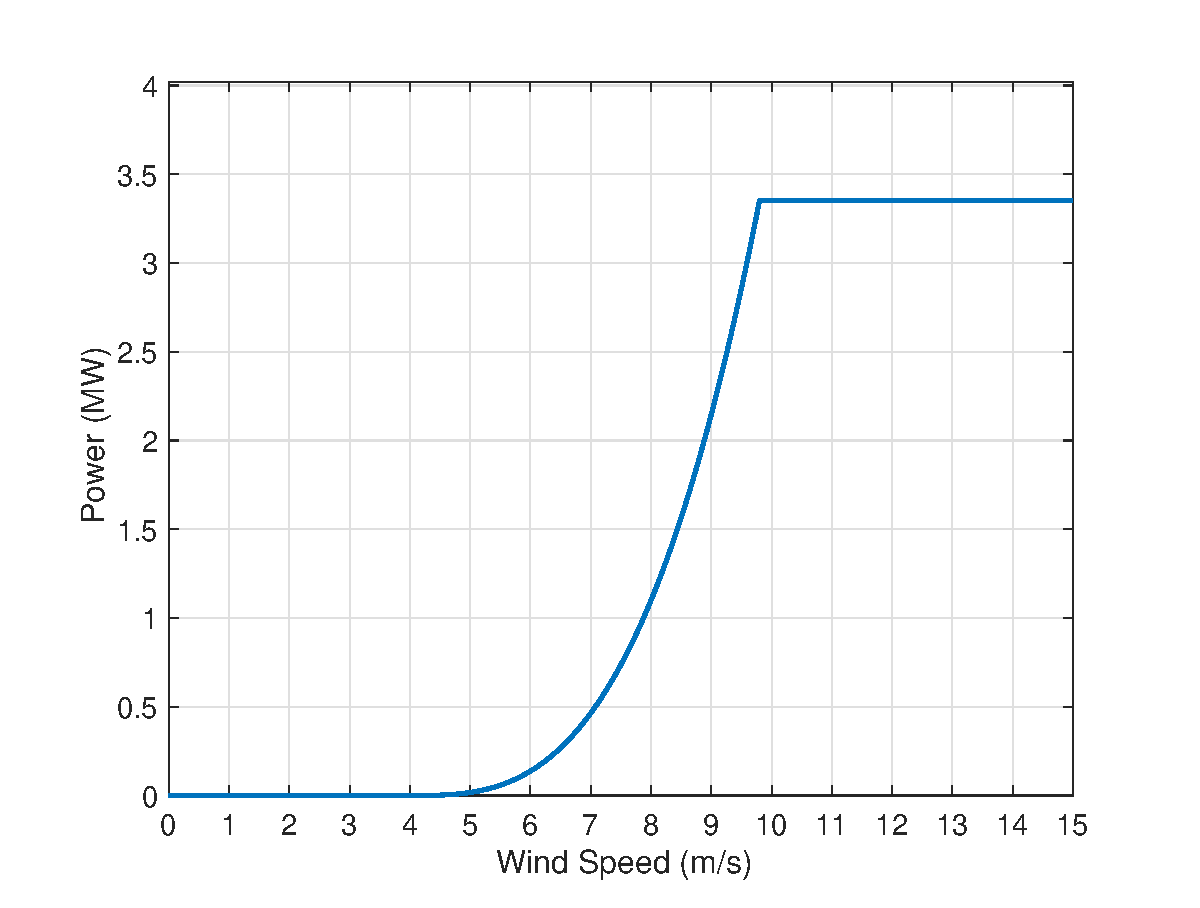
\includegraphics[width=0.75\linewidth]{power-curve.eps}
    \end{figure}

\newpage
\section{Wind Farm Data}
    \subsection{Wind Speed}
        For this scenario, the freestream wind velocity will be constant throughout the farm at $9.8\ \textrm{m/s}$. This is the rated wind speed of the reference turbine described in \cref{App:NREL335MW} used in all farm scenarios, and will enable observation of wake effects.
    
    \subsection{Wind Direction Probability}
    
        For the above specified wind speed, wind direction probability will mimic those found in a geographically linear canyon, using a bi-modal Gaussian distribution. This distribution is defined in  \cref{Eq:freq} and the wind rose is shown below: %in \cref{Fig:freq}.
        
        \begin{align}
        % PDF = \frac{1}{2\pi\sigma^2}\exp{\Bigg[-\frac{(\theta-\mu)^2}{2\sigma^2}\Bigg]}
            F = &w_1\Bigg(\sqrt{\frac{1}{2 \pi \sigma_1^2}}\Bigg)\exp\Bigg(-\frac{(\theta-\mu_1)^2}{2 \sigma_1^2}\Bigg) \nonumber \\
            &+ w_2\Bigg(\sqrt{\frac{1}{2 \pi \sigma_2^2}}\Bigg)\exp\Bigg(-\frac{(\theta-\mu_2)^2}{2 \sigma_2^2}\Bigg) \nonumber \\
            &+ w_2\Bigg(\sqrt{\frac{1}{2 \pi \sigma_2^2}}\Bigg)\exp\Bigg(-\frac{(\theta-\mu_3)^2}{2 \sigma_2^2}\Bigg)
        \label{Eq:freq}
        \end{align}

    The variables for \cref{Eq:freq} are explained in \cref{tab:WindDirProb}:
        \begin{table}[H]
        \centering
        \begin{tabular}{|c|r|l|}
            \hline
             Variable & Value & Definition \\ \hline
            $\theta$ & - & Wind direction where north is $0 \degree$, measured clockwise \\ \hline
            $\mu_1$ & $180\degree$ & First dominant wind direction \\ \hline
            $\mu_2$ & $-10\degree$ & Second dominant wind direction \\ \hline
            $\mu_3$ & $350\degree$ & Second dominant wind direction \\ \hline
            $\sigma_1$ & $20 \degree$ & First standard deviation \\ \hline
            $\sigma_2$ & $40 \degree$ & Second standard deviation \\ \hline
            $w_1$ & $0.5$ & First distribution weight \\ \hline
            $w_2$ & $0.5$ & Second distribution weight \\ \hline
        \end{tabular}
        \caption{Variable definitions for wind direction probability in both case studies}
        \label{tab:WindDirProb}
        \end{table}
    
    The wind rose shown below is a graphical depiction of the frequency from which direction on a compass (in degrees) the wind comes. A greater magnitude in the radial direction from the origin indicates a higher frequency from that direction.
        \begin{figure}[H]
            \centering
            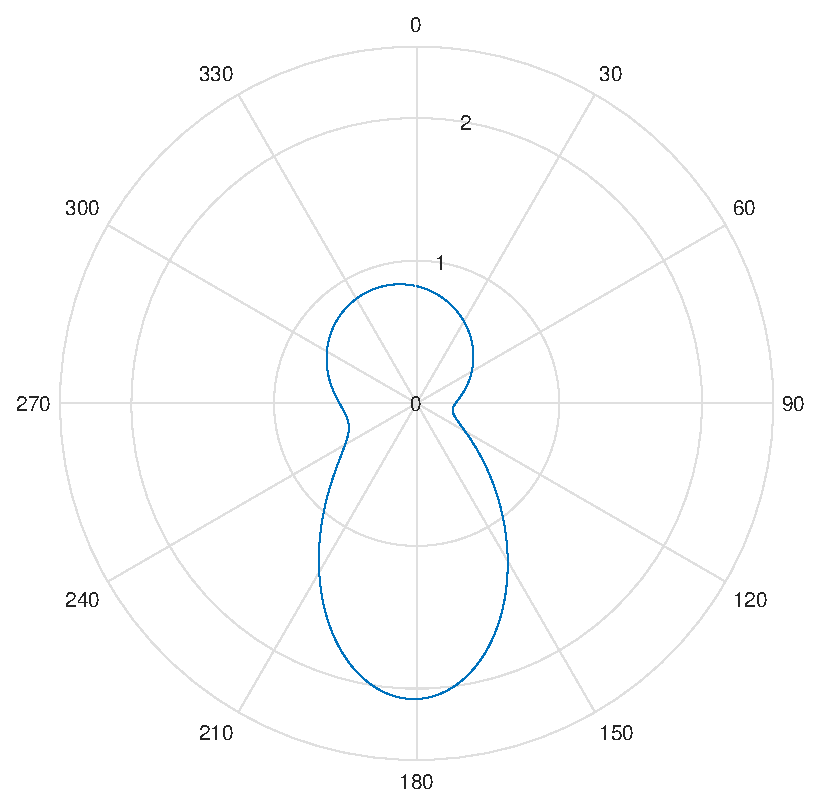
\includegraphics{WindRose.eps}
            \caption{The wind frequency distribution; a bi-modal Gaussian distribution as defined in \cref{Eq:freq}}
            \label{Fig:freq}
        \end{figure}

\newpage
\section{Wake Model Data for Optimization Only Case Study}\label{app:WakeModel}
\subsection{Wake Model}
    For the Optimization Only Case Study (described in \cref{Sec:OptOnly}), we implemented a simplified version of the Bastankhah Gaussian Wake Model \cite{Thomas2018}. The governing equations for the velocity deficit in the waked region, under this case study's implementation are:
    \begin{equation}
        \frac{\Delta U}{U_{\infty}}
        =
        \Bigg(
            1 - \sqrt{
                1 - \frac{C_T}
                    {8\sigma_{y}^{2}/D^2}
                }
        \Bigg)
                \text{exp}\bigg(
                    -0.5\Big(
                        \frac{y-\delta}{\sigma_{y}}
                    \Big)^2
                \bigg)
        \label{Eq:Bast}
    \end{equation}
    \begin{equation}
        \sigma_y = k_y\cdot x + \frac{D}{\sqrt{8}} \\
        \label{Eq:SigY}
    \end{equation}
    
    The relevant variables for \cref{Eq:Bast,Eq:SigY} are defined in \cref{tab:WakeModel}.
    
    \begin{table}[H]
        \centering
        \begin{tabular}{|c|l|l|}
            \hline
             Variable & Value & Definition \\ \hline
            $\frac{\Delta U}{U_{\infty}}$ & - & Wake velocity deficit \\ \hline
            $C_T$ & $\frac{8}{9}$ & Thrust coefficient \\ \hline
            $y-\delta$ & - & Dist. from point of interest to the wake center in cross-stream direction \\ \hline
            $D$ & $130$ m & Turbine diameter \\ \hline
            $\sigma_y$ & \cref{Eq:SigY} & Standard deviation of the wake deficit \\ \hline
            $x$ & - & Downstream dist. from turbine generating wake to turbine of interest \\ \hline
            $k_y$ & 0.0324555 & Variable based on turbulence intensity \cite{Niayifar2016, Thomas2018} \\ \hline
        \end{tabular}
        \caption{Variable definitions for simplified Bastankhah Gaussian Wake Model}
        \label{tab:WakeModel}
    \end{table}
\vspace{-0.25cm}
    No partial wake is accounted for, and hub locations are used for velocity calculations. Turbines feeling multiple wake effects are calculated using the square root of the sum of the squares, as depicted in \cref{Eq:CmbndWake}:
    
    \begin{equation}
    \label{Eq:CmbndWake}
        \bigg(\frac{\Delta U}{U_{\infty}}\bigg)_{cmbnd} = 
            \sqrt{
                \bigg(\frac{\Delta U}{U_{\infty}}\bigg)_{1}^{2} +
                \bigg(\frac{\Delta U}{U_{\infty}}\bigg)_{2}^{2} +
                \bigg(\frac{\Delta U}{U_{\infty}}\bigg)_{3}^{2} +
                \dots}
    \end{equation}

\subsection{AEP}
    Annual Energy Production (AEP) for the Optimization Only Case Study is calculated using \cref{Eq:AEP}, with variable descriptions in \cref{tab:AEP}:
    
    \begin{equation}
        AEP = \omega (\theta) \cdot P (\theta) \cdot 8760 \frac{hrs}{yr}
        \label{Eq:AEP}
    \end{equation}
\vspace{-0.5cm}
    \begin{table}[H]
        \centering
        \begin{tabular}{|c|l|l|}
            \hline
            Variable & Value & Definition \\ \hline
            $\theta$ & $0 \leq \theta \leq 360$ & Wind direction where north is $0 \degree$, measured clockwise \\ \hline
            $\omega(\theta)$ & $0 \leq \omega(\theta) \leq 1$ & Wind frequency, for the given wind direction \\ \hline
            $P(\theta)$ & $0 \leq P(\theta) \leq 3.35 $ & Power (MW), for the given wind direction \\ \hline
        \end{tabular}
        \caption{Variable definitions for AEP calculation}
        \label{tab:AEP}
    \end{table}
    
    Increments of $\theta$ were taken to account for 16 `buckets', or samplings, around the compass. This number was picked since it proved to be past convergence within $1\%$ of truth.

\newpage
\section*{}
\bibliographystyle{unsrt}
\bibliography{references}
\end{document}
